% !TeX program = xelatex
% !TeX encoding = UTF-8
% !TeX TXS-program:compile = txs:///xelatex | txs:///xelatex
\documentclass[aspectratio=169, table, 12pt]{beamer}

% Preamble bersama seluruh slide mata kuliah ini.
% Dipanggil dari slides/sessionXX/sessionXX.tex tepat sesudah baris
% \documentclass[aspectratio=169, table, 12pt]{beamer}
% Paket tambahan yang hanya dibutuhkan satu sesi ditulis di berkas sesi itu.

\usepackage{colortbl}
\usepackage{xcolor}
\usepackage{listings}
\usepackage{tabularx}
\usepackage{booktabs}
\usepackage{tikz}
\usepackage{pgfplots}
\usepackage{fontspec}
\usepackage[english,bahasai]{babel}
\pgfplotsset{compat=1.18}
\usetikzlibrary{arrows.meta, positioning, calc, fit, shapes.geometric,
  shapes.multipart, backgrounds, matrix, chains, trees}

\makeatletter
\def\input@path{{../theme/}}
\makeatother
\graphicspath{{../theme/}{../../figures/}}
% Stub symlink Windows memakai tema cadangan sampai aset institusi tersedia.
\IfFileExists{../theme/beamerthemePradita.sty}{%
  \usetheme{Pradita}
}{%
  \usetheme{Madrid}
  \setmainfont{TeX Gyre Heros}
  \setsansfont{TeX Gyre Heros}
  \setbeamertemplate{navigation symbols}{}
}

\definecolor{praditagreen}{RGB}{37, 113, 71}
\setbeamercolor{structure}{fg=praditagreen}
\setbeamercolor{palette primary}{bg=praditagreen,fg=white}
\setbeamercolor{palette secondary}{bg=praditagreen!80!black,fg=white}
\setbeamercolor{palette tertiary}{bg=praditagreen!60!black,fg=white}
\setbeamerfont{frametitle}{size=\large}
\setbeamertemplate{caption}[numbered]

% Ukuran header mengikuti teks agar judul panjang tidak menabrak logo.
\setbeamercolor{frametitle}{bg=white,fg=black}
\setbeamertemplate{frametitle}{%
  \begin{beamercolorbox}[wd=\paperwidth,sep=0.2cm]{frametitle}
    \begin{minipage}[c]{0.77\paperwidth}
      \raggedright\fontsize{16}{18}\selectfont\bfseries\insertframetitle
      \ifx\insertframesubtitle\empty\else
        \par\small\mdseries\insertframesubtitle
      \fi
    \end{minipage}\hfill
    \begin{minipage}[c]{0.15\paperwidth}
      \IfFileExists{../theme/classFiles/logo_universitas.png}{%
        
\includegraphics[width=\linewidth]{../theme/classFiles/logo_universitas.png}%
      }{}
    \end{minipage}
  \end{beamercolorbox}
}
\setbeamertemplate{footline}{%
  \ifnum\value{framenumber}>1
    \begin{beamercolorbox}[wd=\paperwidth,ht=0.35cm,dp=0.15cm,
      leftskip=0.3cm,rightskip=0.3cm]{palette primary}
      \footnotesize\bfseries\insertframenumber/\inserttotalframenumber
      \hfill IT40813
    \end{beamercolorbox}
  \fi
}
\DeclareRobustCommand{\berkas}[1]{\path{#1}}

% Tema membuat garis tabel berwarna putih. Dikembalikan agar tabel terbaca.
\arrayrulecolor{black}
\setlength{\arrayrulewidth}{0.5pt}

\lstdefinelanguage{yaml}{
  basicstyle=\ttfamily\scriptsize,
  keywordstyle=\color{blue}\bfseries,
  commentstyle=\color{gray}\itshape,
  stringstyle=\color{red},
  showstringspaces=false,
  breaklines=true,
  frame=lines,
  numbers=none,
  backgroundcolor=\color{lightgray!10},
  tabsize=2,
  morecomment=[l]{\#}
}

\lstdefinelanguage{json}{
  basicstyle=\ttfamily\scriptsize,
  stringstyle=\color{red},
  commentstyle=\color{gray},
  breaklines=true,
  showstringspaces=false,
  tabsize=2,
  numbers=none,
  frame=lines,
  backgroundcolor=\color{lightgray!10},
  string=[s]{"}{"}
}

\lstdefinelanguage{bash}{
  keywords={},
  basicstyle=\ttfamily\scriptsize,
  ndkeywords={docker, kubectl, helm, curl, git, terraform},
  ndkeywordstyle=\color{purple}\bfseries,
  sensitive=true,
  commentstyle=\color{gray},
  numbers=none,
  breaklines=true,
  frame=lines,
  backgroundcolor=\color{lightgray!10},
  tabsize=2,
  comment=[l]{\#},
  showstringspaces=false
}

\lstdefinelanguage{http}{
  keywords={GET, POST, PUT, PATCH, DELETE, HEAD, OPTIONS, HTTP},
  basicstyle=\ttfamily\scriptsize,
  keywordstyle=\color{blue}\bfseries,
  sensitive=true,
  numbers=none,
  breaklines=true,
  frame=lines,
  backgroundcolor=\color{lightgray!10},
  tabsize=2,
  showstringspaces=false
}

\subtitle{IT40813 · IT Governance, Risk \& Compliance}
\author{\textbf{Alfa Yohannis}}


% Sampul membatasi judul di panel putih tema rujukan Pradita.
\setbeamertemplate{title page}{%
  \begin{tikzpicture}[remember picture,overlay]
    \node[anchor=north west,inner sep=0pt,text width=8.8cm]
      at ([xshift=1cm,yshift=-3.15cm]current page.north west) {%
        {\small\insertsubtitle\par}\vspace{0.25cm}
        \resizebox{8.8cm}{!}{\begin{minipage}{12cm}
          \raggedright\color{praditagreen}\bfseries\inserttitle
        \end{minipage}}
      };
    \node[anchor=south west,inner sep=0pt]
      at ([xshift=1cm,yshift=1.65cm]current page.south west)
      {\small\insertdate};
    \node[anchor=west,inner sep=0pt,text=white]
      at ([xshift=0.8cm,yshift=0.75cm]current page.south west)
      {\small\insertauthor};
  \end{tikzpicture}
}


\title{\Huge Kelangsungan Bisnis\\ \vspace{10pt} dan Ketahanan Operasional}
\date{Pertemuan 10}

\begin{document}

\frame{\titlepage}

\begin{frame}
  \frametitle{Isi Pertemuan}
  \vspace{14pt}
  \begin{columns}[t]
    \column{0.5\textwidth}
    {\small\tableofcontents[sections={1-4}]}

    \column{0.5\textwidth}
    {\small\tableofcontents[sections={5-8}]}
  \end{columns}
\end{frame}

\begin{frame}{\hfill}
  \centering
  \Huge{\textbf{Server hidup pukul 14.00.\\Mengapa antrean baru\\habis pukul 20.00?}}
\end{frame}

\section{Tujuan dan Konteks}

\begin{frame}{{\Large Tujuan Pembelajaran}}
  \vspace{10pt}
  \begin{itemize}
    \item Melakukan BIA (\textit{Business Impact Analysis}) untuk menentukan layanan kritis beserta
          RTO dan RPO-nya.
    \item Memilih strategi kelangsungan yang sepadan dengan dampak dan biaya.
    \item Merancang skenario latihan krisis yang menguji keputusan, bukan hanya teknologi.
  \end{itemize}
\end{frame}

\begin{frame}{{\Large Masalah: SIMRS Berhenti Enam Jam}}
  \vspace{6pt}
  \small
  \begin{itemize}
    \item Misalkan SIMRS rumah sakit Bekasi berhenti dari pukul 08.00 sampai 14.00.
    \item Petugas menerima pasien dengan kertas, tetapi tidak dapat membaca obat dari unit lain.
    \item Pukul 14.00 server hidup. Antrean dan catatan kertas belum selesai.
    \item Pekerjaan yang ditutup: DSS04 dari Bab 4, 144 uji dari Bab 3, R-05 dari Bab 5.
    \item Hasil kerja: BIA, strategi, dan skenario latihan untuk tonggak C3.
  \end{itemize}
\end{frame}

\begin{frame}{{\Large Alur Keputusan}}
  \vspace{20pt}
  \begin{center}
    \resizebox{0.95\textwidth}{!}{\begin{tikzpicture}[node distance=5mm, kotak/.style={draw, rounded corners, align=center, text width=2.25cm, minimum height=1.2cm, font=\scriptsize}, panah/.style={-{Stealth[length=2mm]}, thick}]
  \node[kotak,fill=praditagreen!15] (t0) {Dampak layanan};
  \node[kotak,fill=blue!8] (t1) [right=of t0] {Target pemulihan};
  \node[kotak,fill=orange!12] (t2) [right=of t1] {Strategi dan sumber daya};
  \node[kotak,fill=green!10] (t3) [right=of t2] {Latihan dan perbaikan};
  \draw[panah] (t0) -- (t1);
  \draw[panah] (t1) -- (t2);
  \draw[panah] (t2) -- (t3);
\end{tikzpicture}
}
  \end{center}
  \vspace{10pt}
  \small Teknologi dipilih sesudah target layanan disepakati, bukan sebelumnya. Rujukan utama: ISO
  22301:2019, NIST SP 800-34 Rev. 1, Peraturan BSSN 1/2024 dan 2/2024, DORA sebagai pembanding.
\end{frame}

\begin{frame}{{\Large Diagram Konsep Bab 10}}
  \centering
  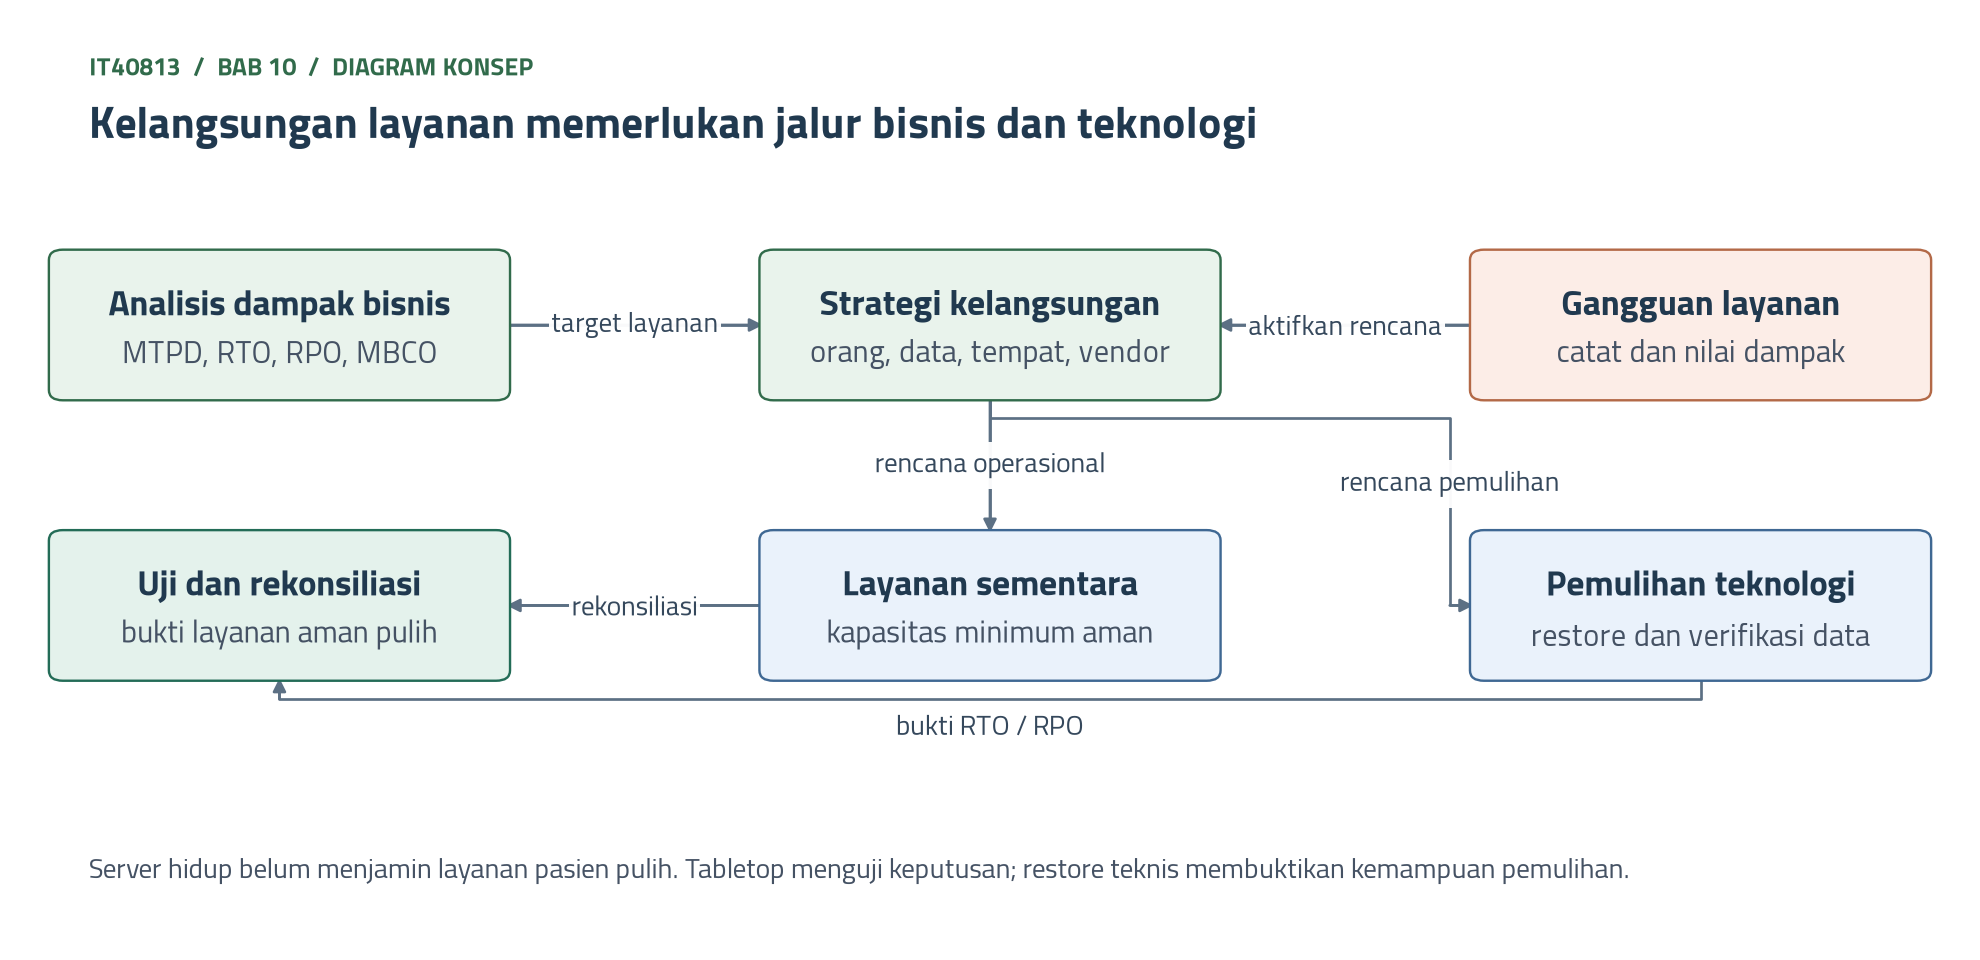
\includegraphics[width=0.96\textwidth,height=0.77\textheight,keepaspectratio]{../../figures/ch10-diagram-konsep.png}
  \label{fig:session10-ilustrasi-bab}
\end{frame}

\section{Tanggung Jawab Direksi}

\begin{frame}{{\Large Tiga Disiplin pada Satu Kejadian}}
  \vspace{4pt}
  \footnotesize
  \begin{tabularx}{\textwidth}{|>{\raggedright\arraybackslash}p{0.2\textwidth}|>{\raggedright\arraybackslash}X|>{\raggedright\arraybackslash}p{0.22\textwidth}|>{\raggedright\arraybackslash}X|}
    \hline
    \textbf{Disiplin} & \textbf{Pertanyaan} & \textbf{Pemimpin} & \textbf{Bukti selesai} \\ \hline
    Manajemen insiden & Apa yang terjadi dan bagaimana dibatasi? & Kepala operasi TI & Kronologi,
    alasan isolasi, hasil pembatasan \\ \hline
    Kelangsungan bisnis & Bagaimana pasien tetap dilayani dengan aman? & Direktur rumah sakit dan
    pemilik layanan & Kapasitas minimum, batas aman \\ \hline
    Pemulihan bencana & Kapan sistem dan data kembali? & Kepala operasi TI & Waktu
    \textit{restore}, titik data, verifikasi \\ \hline
  \end{tabularx}

  \vspace{8pt}
  \small Analogi toko tanpa listrik: teknisi memperbaiki instalasi, pengelola mengatur transaksi
  manual, pemilik memutuskan kapan operasi dihentikan. Laporan ``pulih dalam 90 menit'' hanya
  menjawab satu pertanyaan.
\end{frame}

\begin{frame}{{\Large Siapa Memutuskan}}
  \vspace{4pt}
  \footnotesize
  \begin{tabularx}{\textwidth}{|>{\raggedright\arraybackslash}p{0.24\textwidth}|>{\raggedright\arraybackslash}X|>{\raggedright\arraybackslash}X|}
    \hline
    \textbf{Peran} & \textbf{Keputusan} & \textbf{Bukti} \\ \hline
    Direksi & Toleransi gangguan dan biaya & Persetujuan batas dan anggaran \\ \hline
    Direktur pelayanan & Layanan minimum lintas fasilitas, pengalihan & Catatan pengalihan \\ \hline
    Direktur rumah sakit & Aktivasi operasi manual di lokasi & Waktu aktivasi dan alasannya \\
    \hline
    Pemilik layanan & Kapasitas minimum yang aman & Prosedur manual tervalidasi \\ \hline
    Kepala operasi TI & Urutan pemulihan sistem & Hasil uji pemulihan \\ \hline
  \end{tabularx}

  \vspace{8pt}
  \small Peraturan BSSN 1/2024 Pasal 18 ayat (3): rencana tanggap insiden dan rencana
  keberlangsungan kegiatan disetujui pimpinan organisasi.
\end{frame}

\begin{frame}{{\Large Keputusan yang Tidak Diserahkan kepada Teknisi}}
  \vspace{6pt}
  \small
  \begin{itemize}
    \item Rp120 juta per tahun cukup diputus komite pengarah TI.
    \item Rp480 juta melewati batas Rp400 juta, sehingga naik ke direksi.
    \item Farmasi punya stok, tetapi riwayat obat tidak terbaca. Transaksi manual dibatasi pada
          resep yang dapat diverifikasi. Kaitannya R-11.
    \item Bab 5: gangguan pendaftaran 2 jam per bulan. Enam jam memakai 3 kali batas itu.
    \item Kegagalan mencapai target dieskalasikan sebagai risiko.
  \end{itemize}
\end{frame}

\begin{frame}{{\Large Membandingkan Dua Aturan}}
  \vspace{2pt}
  \scriptsize
  \begin{tabularx}{\textwidth}{|>{\raggedright\arraybackslash}p{0.13\textwidth}|>{\raggedright\arraybackslash}X|>{\raggedright\arraybackslash}X|>{\raggedright\arraybackslash}X|}
    \hline
    \textbf{Pokok} & \textbf{BSSN 1/2024} & \textbf{DORA (pembanding)} & \textbf{Pilihan Medikara
    (misalkan)} \\ \hline
    Pimpinan & Pasal 18 ayat (3): rencana disetujui pimpinan & Pasal 5 ayat (2): tanggung jawab
    akhir pada badan pengelola & Direksi mengesahkan BIA dan rencana \\ \hline
    Target pulih & Lampiran A: capaian dari waktu, jumlah data, fungsi & Pasal 12 ayat (6): target
    waktu dan titik pulih per fungsi & MTPD, RTO, RPO, kapasitas minimum per layanan \\ \hline
    Cadangan & Pasal 18 ayat (3) huruf e: memahami penggunaan rekam cadang & Pasal 12 ayat (3):
    sistem terpisah secara fisik dan logis & Cadangan dan akun terpisah; K-02 \\ \hline
    Frekuensi uji & Pasal 26: berkala; paling sedikit 1 kali dalam 2 tahun bagi penyelenggara IIV &
    Pasal 11 ayat (6): paling sedikit setahun sekali & 144 uji dan 5 \textit{tabletop} per tahun \\
    \hline
  \end{tabularx}

  \vspace{6pt}
  \small DORA berlaku bagi sektor keuangan Uni Eropa, bukan bagi Medikara.
\end{frame}

\section{Sistem Manajemen}

\begin{frame}{{\Large ISO 22301: Sistem, Bukan Resep Perangkat}}
  \vspace{6pt}
  \small
  \begin{itemize}
    \item Lingkup, konteks, tanggung jawab, analisis, strategi, rencana, uji, dan perbaikan.
    \item Analogi latihan kebakaran: peta rapi tidak membuktikan pintu darurat dapat dibuka.
    \item Latihan pada 1 dari 5 rumah sakit dilaporkan 20 persen, atau 1 dari 36 fasilitas sekitar
          2,8 persen.
    \item K-02 meminta tempat berbeda. Alamat berbeda belum tentu mengurangi ancaman bersama.
    \item Naskah ISO berbayar. Rincian klausul dicocokkan ke naskah berlisensi sebelum audit.
  \end{itemize}
\end{frame}

\begin{frame}{{\Large Siklus Pengelolaan Kelangsungan (Misalkan)}}
  \vspace{4pt}
  \footnotesize
  \begin{tabularx}{\textwidth}{|>{\raggedright\arraybackslash}p{0.17\textwidth}|>{\raggedright\arraybackslash}X|>{\raggedright\arraybackslash}X|>{\raggedright\arraybackslash}X|}
    \hline
    \textbf{Tahap} & \textbf{Pertanyaan} & \textbf{Bukti minimum} & \textbf{Contoh Medikara} \\
    \hline
    Rencana & Layanan apa yang dipertahankan? & Ruang lingkup dan BIA & 36 baris BIA, disahkan
    direksi \\ \hline
    Pelaksanaan & Siapa menjalankan alternatif? & Rencana dan daftar kontak & Prosedur korporat
    dengan 36 lampiran \\ \hline
    Evaluasi & Target tercapai atau belum? & Catatan latihan & 144 uji dan 5 \textit{tabletop} per
    tahun \\ \hline
    Perbaikan & Celah mana yang ditutup? & Tindakan, pemilik, tenggat & Uji ulang masuk register
    R-05 \\ \hline
  \end{tabularx}
\end{frame}

\begin{frame}{{\Large DSS04: Delapan Praktik (Misalkan)}}
  \vspace{2pt}
  \scriptsize
  \begin{tabularx}{\textwidth}{|>{\raggedright\arraybackslash}p{0.13\textwidth}|>{\raggedright\arraybackslash}X|>{\raggedright\arraybackslash}X|}
    \hline
    \textbf{Praktik} & \textbf{Inti praktik (diringkas)} & \textbf{Bukti Medikara} \\ \hline
    DSS04.01 & Kebijakan, tujuan, dan ruang lingkup & Ruang lingkup 36 fasilitas disahkan \\ \hline
    DSS04.02 & Menjaga ketahanan bisnis & BIA 36 baris dan pilihan strategi \\ \hline
    DSS04.03 & Mengembangkan dan menerapkan respons & Prosedur korporat, 36 lampiran \\ \hline
    DSS04.04 & Melatih, menguji, dan meninjau rencana & 144 uji dan 5 \textit{tabletop} \\ \hline
    DSS04.05 & Meninjau, memelihara, dan memperbaiki & Tindakan, pemilik, tenggat, uji ulang \\
    \hline
    DSS04.06 & Pelatihan rencana & Petugas manual dilatih dan dicatat \\ \hline
    DSS04.07 & Mengelola pengaturan cadangan & KB-08, K-02, cadangan dan akun terpisah \\ \hline
    DSS04.08 & Tinjauan sesudah pemulihan & Rekonsiliasi disahkan kepala rekam medis \\ \hline
  \end{tabularx}
\end{frame}

\begin{frame}{{\Large Target DSS04: Tingkat 3}}
  \vspace{6pt}
  \small
  \begin{itemize}
    \item 36 prosedur terpisah memakan 288 jam per tahun. Satu korporat dengan 36 lampiran memakan
          112 jam. Selisih 176 jam, atau Rp10,56 juta.
    \item Tingkat 4 menambah Rp180 juta, sedangkan sisa harapan kerugian R-05 hanya Rp40 juta.
    \item Rancangan Bab 8 naik dari Rp600 juta menjadi Rp720 juta per tahun: 4 kali Rp120 juta
          ditambah 4 kali Rp60 juta.
    \item Keputusan tetap di direksi. Kode target baru: T-24.
    \item Rp120 juta hanya kerja proses. Biaya solusi dihitung terpisah.
  \end{itemize}
\end{frame}

\section{Analisis Dampak Bisnis}

\begin{frame}{{\Large Empat Ukuran}}
  \vspace{6pt}
  \small
  \begin{itemize}
    \item MTPD: batas setelah dampak gangguan tidak dapat diterima.
    \item RTO: target waktu pemulihan pada kapasitas yang disepakati.
    \item RPO: titik data yang harus dapat dipulihkan.
    \item MBCO: kapasitas minimum layanan. Bab ini menulisnya kapasitas minimum.
    \item NIST: RTO biasanya lebih pendek daripada MTD, dan RPO bukan bagian MTD.
  \end{itemize}
  \vspace{4pt}
  Analogi kas: kasir jalan lagi dalam 2 jam, buku terakhir 15 menit sebelum gangguan.
\end{frame}

\begin{frame}{{\Large Letak Keempat Ukuran pada Farmasi}}
  \vspace{4pt}
  \begin{center}
    \resizebox{!}{0.74\textheight}{\begin{tikzpicture}[
  font=\scriptsize,
  x=1.75cm,
  y=1cm,
  panah/.style={-{Stealth[length=2mm]}, thick},
  penanda/.style={dashed, gray!70!black, thick}]
  % Baris jalur teknologi
  \node[anchor=east, align=right, text width=1.45cm] at (-0.08,2.05) {Pemulihan\\teknologi};
  \draw[fill=blue!8] (0,1.75) rectangle node[align=center] {\textit{Restore} SIMRS\\uji 90 menit}
    (1.5,2.35);
  \draw[fill=orange!12] (1.5,1.75) rectangle (4,2.35);
  \node[align=center] at (3,2.05) {Verifikasi data\\dan rekonsiliasi};
  % Baris layanan sementara
  \node[anchor=east, align=right, text width=1.45cm] at (-0.08,1.05) {Layanan\\sementara};
  \draw[fill=gray!35] (0,0.75) rectangle node {\tiny Aktivasi} (0.5,1.35);
  \draw[fill=green!10] (0.5,0.75) rectangle (4,1.35);
  \node[align=center] at (3,1.05) {Prosedur manual\\40 resep per jam};
  % Sumbu waktu
  \draw[panah] (-0.85,0) -- (4.55,0);
  \foreach \jam in {0,1,2,3,4} {
    \draw[thick] (\jam,0.08) -- (\jam,-0.08);
    \node[below] at (\jam,-0.06) {\jam\ jam};
  }
  \fill[red!22] (-0.25,-0.1) rectangle (0,0.1);
  % Penanda target
  \draw[very thick, red!60!black] (0,-0.08) -- (0,2.6);
  \node[above, font=\scriptsize\bfseries] at (0,2.6) {Gangguan};
  \draw[penanda] (2,0.08) -- (2,2.6);
  \node[above] at (2,2.6) {RTO layanan dan sistem: 2 jam};
  \draw[penanda] (4,0.08) -- (4,2.6);
  \node[above] at (4,2.6) {MTPD: 4 jam};
  \node[below, align=center] at (-0.42,-0.42) {RPO 15 menit\\(celah data)};
  \draw[gray!70!black] (-0.125,-0.1) -- (-0.3,-0.45);
  \node[anchor=north west, align=left, text width=9.4cm] at (-0.85,-1.2)
    {{\tiny\mdseries Angka farmasi pada satu rumah sakit (pengandaian). RPO berada sebelum gangguan,
    sedangkan RTO dan MTPD berada sesudahnya. Uji 90 menit berada di bawah RTO sistem 120 menit.}};
\end{tikzpicture}
}
  \end{center}
\end{frame}

\begin{frame}{{\Large Langkah Pertama: Dampak Menurut Waktu}}
  \vspace{2pt}
  \footnotesize
  \begin{tabularx}{\textwidth}{|>{\raggedright\arraybackslash}p{0.2\textwidth}|c|c|c|c|c|c|>{\raggedright\arraybackslash}X|}
    \hline
    \textbf{Layanan} & \textbf{1 jam} & \textbf{4 jam} & \textbf{6 jam} & \textbf{12 jam} &
    \textbf{24 jam} & \textbf{48 jam} & \textbf{Cedera berat sejak} \\ \hline
    IGD & 3 & \textbf{4} & 5 & 5 & 5 & 5 & 1 jam \\ \hline
    Farmasi & 2 & \textbf{4} & 4 & 5 & 5 & 5 & 4 jam \\ \hline
    Laboratorium & 2 & \textbf{4} & 4 & 5 & 5 & 5 & 4 jam \\ \hline
    Pendaftaran & 2 & 3 & \textbf{4} & 4 & 5 & 5 & Tidak langsung \\ \hline
    Telekonsultasi & 1 & 2 & 2 & \textbf{4} & 4 & 5 & Tidak langsung \\ \hline
    Klaim BPJS & 1 & 1 & 1 & 2 & 3 & \textbf{4} & Tidak ada \\ \hline
  \end{tabularx}

  \vspace{6pt}
  \small Skala dampak Bab 5. MTPD adalah titik waktu pertama bernilai 4 atau lebih. BIA 36 baris
  memakan 216 jam, atau Rp12,96 juta.
\end{frame}

\begin{frame}{{\Large Contoh Hasil BIA Bekasi (Misalkan)}}
  \vspace{2pt}
  \footnotesize
  \begin{tabularx}{\textwidth}{|>{\raggedright\arraybackslash}p{0.2\textwidth}|>{\raggedright\arraybackslash}X|>{\raggedright\arraybackslash}X|c|c|c|}
    \hline
    \textbf{Layanan} & \textbf{Normal} & \textbf{Minimum} & \textbf{MTPD} & \textbf{RTO} &
    \textbf{RPO} \\ \hline
    IGD & 6 pasien per jam & 6 pasien per jam & 4 jam & 15 menit & 5 menit \\ \hline
    Farmasi & 100 resep per jam & 40 resep per jam & 4 jam & 2 jam & 15 menit \\ \hline
    Laboratorium & 60 hasil per jam & 20 hasil per jam & 4 jam & 2 jam & 15 menit \\ \hline
    Pendaftaran & 40 pasien per jam & 20 pasien per jam & 6 jam & 90 menit & 30 menit \\ \hline
    Telekonsultasi & 40 konsultasi per jam & 10 konsultasi per jam & 12 jam & 6 jam & 60 menit \\
    \hline
    Klaim BPJS & 300 klaim per hari & 100 klaim per hari & 48 jam & 24 jam & 4 jam \\ \hline
  \end{tabularx}

  \vspace{6pt}
  \small MTPD IGD 4 jam adalah pengandaian latihan: batas SIMRS boleh berhenti selama jalur manual
  berjalan penuh, bukan batas IGD boleh berhenti. Angka klinis bukan standar pelayanan dan harus
  divalidasi pihak yang berwenang.
\end{frame}

\begin{frame}{{\Large Dua Hal yang Sering Tertukar}}
  \vspace{6pt}
  \small
  \begin{itemize}
    \item RTO layanan: kapan pasien dilayani lagi pada kapasitas minimum, lewat jalur apa pun.
    \item RTO sistem: kapan SIMRS dan datanya kembali. Di sini $240 - 120 = 120$ menit.
    \item Uji 150 menit gagal 30 menit, walaupun formulir kertas berjalan sejak menit ke-30.
    \item Batas Bab 5 kumulatif, 2 jam per bulan. MTPD per kejadian, 6 jam pada pendaftaran. RTO
          pendaftaran 90 menit menyisakan 30 menit.
    \item Cadangan malam: sampai 1.200 resep hilang, 60 jam kerja. RPO 15 menit: 25 resep, 75 menit.
  \end{itemize}
\end{frame}

\begin{frame}{{\Large Langkah Kedua: Ketergantungan}}
  \vspace{2pt}
  \begin{center}
    \resizebox{!}{0.76\textheight}{\begin{tikzpicture}[
  font=\scriptsize,
  layanan/.style={draw, rounded corners, fill=blue!8, minimum width=2.25cm, minimum height=0.56cm,
    align=center},
  sistem/.style={draw, rounded corners, fill=orange!12, minimum width=2.6cm, minimum height=0.8cm,
    align=center},
  pendukung/.style={draw, rounded corners, fill=green!10, minimum width=3.1cm, minimum height=0.8cm,
    align=center},
  masalah/.style={draw, rounded corners, fill=red!22, minimum width=3.1cm, minimum height=0.8cm,
    align=center},
  panah/.style={-{Stealth[length=2mm]}, thick}]
  \node[font=\scriptsize\bfseries] at (0,0.65) {Layanan};
  \node[font=\scriptsize\bfseries] at (4.1,0.65) {Sistem};
  \node[font=\scriptsize\bfseries] at (8.4,0.65) {Pendukung};
  \node[layanan] (igd) at (0,0) {IGD};
  \node[layanan] (farmasi) at (0,-0.8) {Farmasi};
  \node[layanan] (lab) at (0,-1.6) {Laboratorium};
  \node[layanan] (daftar) at (0,-2.4) {Pendaftaran};
  \node[layanan] (klaim) at (0,-3.2) {Klaim BPJS};
  \node[layanan] (tele) at (0,-4.0) {Telekonsultasi};
  \node[sistem] (simrs) at (4.1,-1.2) {SIMRS dan\\identitas pasien};
  \node[sistem] (integrasi) at (4.1,-2.75) {Integrasi BPJS};
  \node[sistem] (medikara) at (4.1,-4.0) {Medikara+ (V-01)};
  \node[pendukung] (jaringan) at (8.4,0) {Jaringan dan listrik};
  \node[pendukung] (cadangan) at (8.4,-1.3) {Cadangan pada\\penyedia cloud (V-02)};
  \node[masalah] (identitas) at (8.4,-2.75) {Layanan identitas\\bersama};
  \node[pendukung] (pesan) at (8.4,-4.1) {Penyedia pesan\\bersama};
  \draw[panah] (igd.east) -- (simrs.west);
  \draw[panah] (farmasi.east) -- (simrs.west);
  \draw[panah] (lab.east) -- (simrs.west);
  \draw[panah] (daftar.east) -- (simrs.west);
  \draw[panah] (klaim.east) -- (integrasi.west);
  \draw[panah] (tele.east) -- (medikara.west);
  \draw[panah] (integrasi.north) -- (simrs.south);
  \draw[panah] (simrs.east) -- (jaringan.west);
  \draw[panah] (simrs.east) -- (cadangan.west);
  \draw[panah] (simrs.east) -- (identitas.west);
  \draw[panah] (cadangan.south) -- (identitas.north);
  \draw[panah] (medikara.east) -- (identitas.west);
  \draw[panah] (medikara.east) -- (pesan.west);
  \node[anchor=north west, align=left, text width=11cm] at (-1.15,-4.75)
    {{\tiny\mdseries Panah berarti bergantung pada. Merah: titik kegagalan bersama menurut peta Bab 9.
    Rancangan target, seluruhnya pengandaian dan perlu dibuktikan lewat kontrak serta uji.}};
\end{tikzpicture}
}
  \end{center}
\end{frame}

\begin{frame}{{\Large Dua Hitungan Ketergantungan dan Prioritas}}
  \vspace{6pt}
  \small
  \begin{itemize}
    \item Layanan identitas dijanjikan pulih 8 jam. \textit{Restore} 90 menit baru dapat dimulai
          sesudahnya: 9,5 jam, atau 5,5 jam di atas MTPD.
    \item 144 uji dengan akun yang sama tidak akan menemukan selisih ini.
    \item Kontrak V-01 24 jam, RTO telekonsultasi 6 jam. Selisih 18 jam ditutup telepon atau tawar
          ulang. Sekitar 933 janji temu terganggu.
    \item Prioritas: identitas pasien, lalu IGD, farmasi, dan laboratorium.
    \item Disusul pendaftaran, telekonsultasi, dan klaim BPJS.
  \end{itemize}
\end{frame}

\begin{frame}{{\Large Kasus Medikara: Antrean Enam Jam di Bekasi}}
  \vspace{2pt}
  \begin{center}
    \resizebox{!}{0.76\textheight}{\begin{tikzpicture}[font=\scriptsize, x=0.72cm, y=0.0167cm]
  % Garis bantu dan sumbu: satu satuan x adalah satu jam, satu satuan y adalah satu pasien
  \foreach \nilai in {60,120,180,240} {
    \draw[gray!35] (0,\nilai) -- (12,\nilai);
    \node[left] at (0,\nilai) {\nilai};
  }
  \draw[thick] (0,0) -- (12,0);
  \node[left] at (0,0) {0};
  \foreach \posisi/\jam in {0/08.00,2/10.00,4/12.00,6/14.00,8/16.00,10/18.00,12/20.00} {
    \draw (\posisi,0) -- (\posisi,-5);
    \node[below] at (\posisi,-5) {\jam};
  }
  \node[anchor=south west] at (-0.6,256) {Pasien menunggu pendaftaran};
  % Penanda saat SIMRS kembali
  \draw[dashed, gray!70!black, thick] (6,0) -- (6,272);
  \node[above] at (6,272) {SIMRS pulih};
  % Seri tanpa prosedur manual
  \draw[orange!70!black, thick, dashed] (0,0) -- (6,240) -- (12,120);
  \fill[orange!70!black] (6,240) circle (1.6pt) (12,120) circle (1.6pt);
  \node[anchor=west] at (6.1,246) {Tanpa manual: 240 pasien};
  \node[anchor=west, align=left] at (12.1,120) {120 pasien\\masih menunggu};
  % Seri dengan prosedur manual
  \draw[blue!60!black, thick] (0,0) -- (6,120) -- (12,0);
  \fill[blue!60!black] (6,120) circle (1.6pt) (12,0) circle (1.6pt);
  \node[align=left, anchor=north west] at (6.1,62) {Dengan manual:\\120 pasien};
  \node[anchor=west, align=left] at (12.1,8) {Antrean\\habis};
  % Legenda
  \draw[blue!60!black, thick] (0,-48) -- (1,-48);
  \node[anchor=west] at (1.05,-48) {Dengan prosedur manual};
  \draw[orange!70!black, thick, dashed] (6.1,-48) -- (7.1,-48);
  \node[anchor=west] at (7.15,-48) {Tanpa prosedur manual};
  \node[anchor=north west, align=left, text width=9.6cm] at (-0.6,-62)
    {{\tiny\mdseries Pengandaian rumah sakit Bekasi: 40 pasien datang per jam, manual 20 per jam,
    tanpa manual 0 per jam, sesudah SIMRS pulih 60 per jam.}};
\end{tikzpicture}
}
  \end{center}
\end{frame}

\begin{frame}{{\Large Kasus Medikara: Membaca Hitungan}}
  \vspace{6pt}
  \small
  \begin{itemize}
    \item Enam jam: 240 pasien datang, 120 terlayani, 120 menunggu.
    \item Sesudah pulih, antrean turun 20 per jam dan habis pukul 20.00. Tanpa manual, masih tersisa
          120 pasien.
    \item Rekonsiliasi: 120 pendaftaran 10 jam, 240 resep 12 jam, total 22 jam kerja.
    \item Enam jam melewati MTPD farmasi, IGD, dan laboratorium sebesar 2 jam.
    \item Pengalihan sebagian layanan semestinya mulai sejak jam ke-4.
  \end{itemize}
\end{frame}

\section{Strategi Kelangsungan}

\begin{frame}{{\Large Dua Jalur Strategi (Misalkan)}}
  \vspace{2pt}
  \scriptsize
  \begin{tabularx}{\textwidth}{|>{\raggedright\arraybackslash}p{0.17\textwidth}|>{\raggedright\arraybackslash}X|>{\raggedright\arraybackslash}X|>{\raggedright\arraybackslash}p{0.2\textwidth}|}
    \hline
    \textbf{Layanan} & \textbf{Rencana operasional} & \textbf{Rencana pemulihan} & \textbf{Risiko
    sisa} \\ \hline
    IGD & Triase kertas, gelang identitas, pengalihan & Salinan baca saja riwayat alergi, KB-04 &
    Data lintas unit lambat; R-11 \\ \hline
    Farmasi & Resep kertas yang dapat diverifikasi & Cadangan terpisah, pemulihan prioritas & Resep
    tanpa riwayat tertahan \\ \hline
    Laboratorium & Hasil kritis lewat telepon, pembacaan ulang & Pemulihan antarmuka alat & Salah
    identitas \\ \hline
    Pendaftaran & Formulir kertas, daftar jadwal harian & Identitas pasien lebih dulu & Antrean,
    rekonsiliasi \\ \hline
    Telekonsultasi & Telepon, 10 konsultasi per jam & Kontrak V-01, uji ekspor tahunan & Janji temu
    tertunda \\ \hline
    Klaim BPJS & Tunda, lalu 100 klaim per hari & Pulih sesudah layanan klinis & Penumpukan
    administrasi \\ \hline
  \end{tabularx}

  \vspace{6pt}
  \small Orang, data, tempat, dan vendor menghasilkan layanan sementara dan pemulihan teknologi.
\end{frame}

\begin{frame}{{\Large Membaca Penelitian: Prosedur Manual}}
  \vspace{6pt}
  \small
  \begin{itemize}
    \item Larsen dan rekan (2018): 76 dari 80.381 laporan insiden menyebut rekam medis elektronik
          yang berhenti.
    \item 37 laporan (48,7 persen) laboratorium; 11 laporan (14,5 persen) obat.
    \item 35 laporan (46 persen): prosedur tidak diikuti atau tidak tersedia.
    \item 21 laporan (27,6 persen): prosedur berjalan.
    \item Bukan peluang Medikara. Nilainya pada arah perhatian: laboratorium, obat, identitas.
  \end{itemize}
\end{frame}

\begin{frame}{{\Large Replikasi dan Cadangan}}
  \vspace{6pt}
  \small
  \begin{itemize}
    \item Replikasi menyalin perubahan dengan cepat, termasuk kerusakan.
    \item Cadangan terpisah menyimpan titik waktu, tetapi pemulihannya dapat lebih lambat.
    \item Analogi: mesin fotokopi ke kantor cabang dan arsip di lemari terkunci.
    \item Replikasi 5 menit: RPO 5 menit berlaku untuk kegagalan perangkat, bukan
          \textit{ransomware}.
    \item Akun yang sama dapat merusak kedua salinan. Tempat berbeda belum cukup bila aksesnya sama.
  \end{itemize}
\end{frame}

\begin{frame}{{\Large Tiga Opsi untuk Lima Rumah Sakit per Tahun (Misalkan)}}
  \vspace{2pt}
  \scriptsize
  \begin{tabularx}{\textwidth}{|>{\raggedright\arraybackslash}p{0.22\textwidth}|>{\raggedright\arraybackslash}p{0.13\textwidth}|>{\raggedright\arraybackslash}X|>{\raggedright\arraybackslash}X|>{\raggedright\arraybackslash}X|}
    \hline
    \textbf{Ukuran} & \textbf{Target} & \textbf{A. Manual terkontrol} & \textbf{B. Manual dan
    pemulihan prioritas} & \textbf{C. Replikasi aktif} \\ \hline
    Biaya per tahun & & Rp120 juta & Rp480 juta & Rp6 miliar \\ \hline
    Kapasitas manual farmasi & 40 per jam & 20 per jam & 40 per jam & 40 per jam \\ \hline
    SIMRS pulih & 120 menit & 480 menit & 90 menit & Mendekati nol; 90 menit bila data rusak \\
    \hline
    Titik data & 15 menit & Sampai 24 jam & 10 menit & Mendekati nol; 10 menit bila data rusak \\
    \hline
    Harapan kerugian R-05 & & Rp200 juta & Rp40 juta & Rp40 juta \\ \hline
    Biaya ditambah kerugian & & Rp320 juta & Rp520 juta & Rp6,04 miliar \\ \hline
    Hasil & & Ditolak & Layak bersyarat & Ditolak \\ \hline
  \end{tabularx}
\end{frame}

\begin{frame}{{\Large Pilihan A dan B: Tradeoff yang Nyata}}
  \vspace{6pt}
  \small
  \begin{itemize}
    \item A lebih murah Rp200 juta per tahun. Tambahan Rp360 juta hanya menurunkan harapan kerugian
          Rp160 juta.
    \item A melanggar batas 2 persen dan kapasitas minimum. Selisih itu harga memenuhi batas.
    \item C menelan 12,5 kali B dan melewati batas direksi Rp5 miliar.
    \item Persetujuan bersyarat: Rp360 juta dua tahap, 5 dari 5 rumah sakit lulus uji, 9 uji akun
          terpisah berhasil.
    \item Harapan kerugian tidak mengukur cedera pasien.
  \end{itemize}
\end{frame}

\section{Insiden dan Krisis}

\begin{frame}{{\Large Tiga Tingkat Eskalasi}}
  \vspace{12pt}
  \begin{center}
    \resizebox{0.95\textwidth}{!}{\begin{tikzpicture}[
  font=\scriptsize,
  tingkat/.style={draw, rounded corners, align=center, text width=3.05cm, minimum height=1.25cm},
  catatan/.style={align=center, text width=3.05cm},
  panah/.style={-{Stealth[length=2mm]}, thick}]
  \node[tingkat, fill=blue!8] (insiden) at (0,0)
    {\textbf{Insiden siber}\\Tim tanggap organisasi\\Kepala operasi TI};
  \node[tingkat, fill=orange!12] (krisis) at (4.3,0)
    {\textbf{Krisis organisasi}\\Istilah internal Medikara\\Direksi memimpin};
  \node[tingkat, fill=red!22] (nasional) at (8.6,0)
    {\textbf{Krisis Siber}\\Situasi darurat nasional\\Presiden menetapkan};
  \draw[panah] (insiden) -- (krisis);
  \draw[panah] (krisis) -- (nasional);
  \node[catatan, below=2mm of insiden]
    {Batasi, catat kronologi, nilai dampak. Lapor bila paling sedikit berisiko tinggi};
  \node[catatan, below=2mm of krisis]
    {Pemicu: RTO terlewat, lebih dari satu rumah sakit, atau risiko cedera berat};
  \node[catatan, below=2mm of nasional]
    {Bukan keputusan Medikara. Sebagai PSE, Medikara menindaklanjuti peringatan dini};
  \node[anchor=north west, align=left, text width=11.4cm] at (-1.55,-2.75)
    {{\tiny\mdseries Pemicu krisis organisasi adalah pengandaian Medikara. Definisi dan penetapan Krisis
    Siber mengikuti Peraturan BSSN 2/2024 Pasal 1 angka 3 dan Pasal 13 ayat (2).}};
\end{tikzpicture}
}
  \end{center}
  \vspace{4pt}
  \small Rumah sakit tidak dapat menyatakan Krisis Siber. Peringatan dini: PSE menindaklanjuti dan
  melapor setiap 2 jam, atau 6 laporan dalam 12 jam layanan.
\end{frame}

\begin{frame}{{\Large Komunikasi dan Pemberitahuan}}
  \vspace{6pt}
  \small
  \begin{itemize}
    \item Sampaikan yang diketahui, dampak layanan, tindakan sementara, dan waktu pembaruan.
    \item Pukul 09.00: cakupan dan jadwal diumumkan, penyebab yang belum terverifikasi tidak.
    \item Selasa 09.15 indikasi data keluar. Jam ke-60: Kamis 21.15.
    \item Batas terluar $3 \times 24$ jam: Jumat 09.15. K-05 vendor 12 jam: Selasa 21.15.
    \item SIMRS pulih pukul 14.00 tidak menggeser ketiga batas itu.
  \end{itemize}
\end{frame}

\begin{frame}{{\Large Catatan Keputusan Krisis (Misalkan)}}
  \vspace{4pt}
  \footnotesize
  \begin{tabularx}{\textwidth}{|>{\raggedright\arraybackslash}X|>{\raggedright\arraybackslash}X|>{\raggedright\arraybackslash}p{0.2\textwidth}|>{\raggedright\arraybackslash}X|}
    \hline
    \textbf{Keputusan} & \textbf{Pemilik} & \textbf{Target waktu} & \textbf{Bukti} \\ \hline
    Isolasi sistem & Kepala operasi TI & 15 menit & Alasan dan waktu isolasi \\ \hline
    Operasi manual & Direktur rumah sakit & 20 menit & Kapasitas dan batas aman \\ \hline
    Pengalihan pasien & Direktur pelayanan & 30 menit & Fasilitas penerima, kapasitas \\ \hline
    Pernyataan publik & Direktur utama & 60 menit & Fakta terverifikasi, jadwal \\ \hline
    Pemberitahuan & Fungsi hukum, petugas pelindungan data & Jam ke-60, terluar $3 \times 24$ jam &
    Dasar, penerima, waktu kirim \\ \hline
  \end{tabularx}
\end{frame}

\begin{frame}{{\Large Membaca Penelitian: Pengalihan Pasien}}
  \vspace{6pt}
  \small
  \begin{itemize}
    \item Dameff dan rekan (2023): serangan Mei 2021 pada 4 rumah sakit; 2 IGD tetangga ditelaah.
    \item Pasien harian 218,4 menjadi 251,4 (15,1 persen); ambulans 1.741 menjadi 2.354 (35,2
          persen).
    \item Median waktu masuk ruang periksa 21 menjadi 31 menit; pulang sebelum dilayani 158 menjadi
          360.
    \item Observasional pada satu wilayah. Angkanya tidak disalin ke Medikara.
    \item Misalkan IGD Bekasi mengalihkan 3 pasien per jam ke 2 IGD: tiap penerima naik 25 persen.
  \end{itemize}
\end{frame}

\section{Latihan dan Pengujian}

\begin{frame}{{\Large Jenis Pengujian dan Batas Buktinya}}
  \vspace{4pt}
  \footnotesize
  \begin{tabularx}{\textwidth}{|>{\raggedright\arraybackslash}p{0.22\textwidth}|>{\raggedright\arraybackslash}X|>{\raggedright\arraybackslash}X|}
    \hline
    \textbf{Metode} & \textbf{Yang diuji} & \textbf{Yang belum dibuktikan} \\ \hline
    \textit{Tabletop} & Wewenang dan keputusan & Kecepatan pemulihan server \\ \hline
    Latihan fungsional & Peran dan prosedur satu fungsi & Fungsi lain, data lintas unit \\ \hline
    Uji teknis & Waktu dan integritas data & Kesiapan seluruh petugas \\ \hline
    Latihan terpadu & Layanan minimum lintas unit & Semua skenario masa depan \\ \hline
  \end{tabularx}

  \vspace{8pt}
  \small Uji 150 menit terhadap RTO 120 menit: selisih 30 menit masuk register dan IT40713.
  Keputusan manual 35 menit terhadap target 20 menit: selisih 15 menit menjadi temuan.
\end{frame}

\begin{frame}{{\Large Mengisi 144 Uji Pemulihan}}
  \vspace{2pt}
  \footnotesize
  \begin{tabularx}{\textwidth}{|>{\raggedright\arraybackslash}X|c|c|c|c|c|}
    \hline
    \textbf{Triwulan pertama} & \textbf{Uji} & \textbf{Lulus} & \textbf{Lewat RTO} & \textbf{Data
    gagal} & \textbf{Persen} \\ \hline
    5 rumah sakit & 5 & 3 & 1 & 1 & 60,0 \\ \hline
    31 fasilitas lain & 31 & 26 & 4 & 1 & 83,9 \\ \hline
    Total & 36 & 29 & 5 & 2 & 80,6 \\ \hline
  \end{tabularx}

  \vspace{6pt}
  \small
  \begin{itemize}
    \item 144 uji dan 432 jam tetap. Hanya 20 uji menyentuh SIMRS rumah sakit.
    \item 108 uji biasa dan 36 uji akun terpisah, atau 25 persen.
    \item Dua data gagal berasal dari 9 uji akun terpisah. Angka lulus bukan peluang R-05.
  \end{itemize}
\end{frame}

\begin{frame}{{\Large Skenario Tabletop dan Contoh Hasil (Misalkan)}}
  \vspace{2pt}
  \scriptsize
  \begin{tabularx}{\textwidth}{|>{\raggedright\arraybackslash}p{0.08\textwidth}|>{\raggedright\arraybackslash}X|>{\raggedright\arraybackslash}p{0.22\textwidth}|c|c|}
    \hline
    \textbf{Waktu} & \textbf{Informasi dan keputusan} & \textbf{Pemilik} & \textbf{Target} &
    \textbf{Aktual} \\ \hline
    08.00 & SIMRS tidak dapat dibuka. Siapa memimpin? & Kepala operasi TI & 10 & 8 \\ \hline
    08.15 & Berkas terenkripsi di tiga unit. Apa yang diisolasi? & Kepala operasi TI & 15 & 15 \\
    \hline
    08.15 & Layanan terganggu. Kapan manual aktif? & Direktur rumah sakit & 20 & 35 \\ \hline
    08.30 & Cadangan belum tervalidasi. Strategi apa dipilih? & Direktur pelayanan & 30 & 25 \\
    \hline
    08.45 & Vendor tidak dapat dihubungi. Kapan jalur lain aktif? & Kepala operasi TI & 15 & 40 \\
    \hline
    09.00 & Media menanyakan kebocoran. Apa yang diumumkan? & Direktur utama & 60 & 50 \\ \hline
    09.15 & Indikasi data keluar. Kapan proses pemberitahuan dimulai? & Fungsi hukum & 30 & 45 \\
    \hline
  \end{tabularx}

  \vspace{4pt}
  \small Diskusi 45 menit, evaluasi 15 menit. Tanpa menyentuh sistem nyata dan tanpa data pasien.
\end{frame}

\begin{frame}{{\Large Kasus Medikara: Membaca Hasil Tabletop}}
  \vspace{6pt}
  \small
  \begin{itemize}
    \item Empat dari tujuh keputusan tepat waktu, sekitar 57 persen. Total terlambat 55 menit.
    \item Manual +15: daftar kewenangan. Vendor +25: satu nomor kontak. Hukum +15: baru diundang.
    \item Tindakan dalam 14 sampai 30 hari, uji ulang dalam 60 hari.
    \item Keputusan 08.30 tepat waktu, tetapi memakai cadangan yang belum tervalidasi.
    \item Lima rumah sakit: 35 jam per tahun. Beban Bab 8 tahun pertama 1.443 jam, sekitar 0,75
          orang penuh waktu.
  \end{itemize}
\end{frame}

\section{Penutup}

\begin{frame}{{\Large Aktivitas: BIA dan Strategi Kelangsungan Layanan}}
  \vspace{4pt}
  \small
  \begin{itemize}
    \item Nilai dampak 5 sampai 7 layanan. Tetapkan MTPD, RTO, RPO, dan kapasitas minimum.
    \item Bandingkan strategi dua layanan kritis menurut biaya, asumsi, dan risiko sisa.
    \item Jalankan \textit{tabletop}. Catat waktu, dasar bukti, tindakan, dan uji ulang.
    \item Peran: kesehatan atau operasional, analis teknologi, analis risiko, pemilik konteks.
    \item Luaran masuk C3, selaras dengan IT40713. Berkas: \texttt{sources/chapter10/README.md}.
  \end{itemize}
\end{frame}

\begin{frame}{{\Large Ringkasan}}
  \vspace{4pt}
  \small
  \begin{itemize}
    \item Direksi menetapkan toleransi. DSS04 tingkat 3, rancangan Bab 8 menjadi Rp720 juta.
    \item BIA: MTPD 4 jam menurunkan RTO sistem 120 menit. Ketergantungan dapat mengalahkan target.
    \item Strategi dua jalur. Opsi B Rp200 juta lebih mahal per tahun untuk memenuhi batas 2 persen.
    \item Krisis Siber ditetapkan Presiden. Pemulihan tidak menggeser batas $3 \times 24$ jam.
    \item Layanan pulih ketika pasien dapat dilayani secara aman pada kapasitas yang disepakati.
  \end{itemize}
\end{frame}

\begin{frame}{{\Large Latihan}}
  \vspace{4pt}
  \small
  \begin{enumerate}
    \item Jelaskan perbedaan RTO dan RPO dengan contoh layanan farmasi rumah sakit.
    \item Mengapa RTO untuk semua layanan tidak boleh ditetapkan nol? Kaitkan dengan biaya dan
          \textit{risk appetite}.
    \item Rancang tiga pertanyaan keputusan yang harus dijawab direksi dalam latihan
          \textit{tabletop} serangan \textit{ransomware}.
  \end{enumerate}
  \vspace{6pt}
  Gunakan tabel contoh dan lembar hasil pada modul untuk membela alasan.
\end{frame}

\end{document}
